\documentclass[sigconf]{acmart}
\usepackage{placeins}

\AtBeginDocument{%
  \providecommand\BibTeX{{%
    Bib\TeX}}}

\settopmatter{printacmref=false}

\makeatletter
\def\@copyrightpermission{\relax}
\def\@copyrightowner{\relax}
\makeatother

\acmConference[Fungi-On]{}{Nov 16, 2023}{PRI course, M.EIC}

\begin{document}

\title{Fungi-On: An Information Search System for Fungi Taxonomy and Field Observations in the Iberian Peninsula}

\author{Guilherme Sequeira}
\email{up202004648@up.pt}
\affiliation{%
  \institution{Faculty of Engineering, University of Porto}
  \city{Porto}
  \country{Portugal}
}

\author{Pedro Nunes}
\email{up202004714@up.pt}
\affiliation{%
  \institution{Faculty of Engineering, University of Porto}
  \city{Porto}
  \country{Portugal}
}

\author{Pedro Ramalho}
\email{up202004715@up.pt}
\affiliation{%
  \institution{Faculty of Engineering, University of Porto}
  \city{Porto}
  \country{Portugal}
}

\renewcommand{\shortauthors}{Guilherme Sequeira, Pedro Nunes, and Pedro Ramalho}

\begin{abstract}
  %This report details the development of the first milestone of our project, developed as part of the Information Processing and Retrieval curricular unit. This milestone encompasses the selection, preparation, and characterization of a dataset. It will result in a reproducible pipeline for data processing, the output of which is a collection of documents that will act as a base for the subsequent milestones. We have selected a dataset which compiles occurrences of different species of Fungi in Portugal and Spain.

  This project aims to introduce an information search system on fungi, developed on top of data collected from publicly accessible sources. The development process includes preparation and processing of this data to ensure it's quality and relevance. This search system is expected to fulfill the various information needs of a broad range of end users interested in knowing more about the fungal diversity and distribution in the context of the Iberian Peninsula. 
\end{abstract}

% This code was generated by the tool available at http://dl.acm.org/ccs.cfm
\begin{CCSXML}
<ccs2012>
<concept>
<concept_id>10002951.10003317</concept_id>
<concept_desc>Information systems~Information retrieval</concept_desc>
<concept_significance>500</concept_significance>
</concept>
</ccs2012>
\end{CCSXML}
\ccsdesc[500]{Information systems~Information retrieval}

% keywords
\keywords{Fungi, Fungus, Dataset, Information Processing, Information Retrieval}

%%
%% This command processes the author and affiliation and title
%% information and builds the first part of the formatted document.
\maketitle

% Section 1: Introduction
\section{Introduction}

In this study we address the intersection of information retrieval and mycology, focusing on the extensive vital class of organisms, fungi. Fungi play diverse roles in ecosystems, from supporting plant life to providing valuable pharmaceutical compounds.

To streamline data access, we leverage the Global Biodiversity Information Facility (GBIF) \cite{GBIF}, an international data infrastructure committed to open access to a broad array of datasets \cite{Dataset} from multiple authoritative sources. GBIF enables precise searches and the retrieval of curated data subsets. With these resources, our goal is to develop a specialized search engine tailored to fungal species and occurrences. We concentrate our efforts on specific geographical regions, namely Portugal and Spain, to compile a comprehensive dataset. Additionally, we plan to utilize Application Programming Interfaces (APIs) for supplementary data collection. 

\section{Milestone 1 - Data preparation}

The first milestone encompasses the selection, preparation, and characterization of a dataset. It results in a reproducible pipeline for data processing, the output of which is a collection of documents that will serve as a base for the subsequent milestones.

% Section 2: Data Processing
\subsection{Data Processing and Preparation}

This subsection outlines our systematic approach to collecting, cleansing, and structuring data on fungal species and observations. In the following subsubsections you may find a detailed explanation of each of these tasks, as well as a conceptual data model and a reproducible pipeline.

\subsubsection{\textbf{Data Collection}}

As previously mentioned, structured data was sourced from GBIF, a reputable international data infrastructure. Two primary datasets were acquired: \texttt{occurrences}, which contains information regarding fungal species occurrences, and \texttt{multimedia}, which provides visual representations such as images and pictures associated with these occurrences. Both datasets were available in tab-separated values format. The \texttt{occurrences} dataset comprised over 700,000 rows and had a file size of 784 MB, whilst the \texttt{multimedia} dataset contained over 120,000 rows and had a file size of 28 MB. The data obtained from GBIF belong to different datasets, each with one of three licenses: \texttt{CC0 1.0}, \texttt{CC BY-NC 4.0} and \texttt{CC BY 4.0}, all of which permit the copy and redistribute the material in any medium or format and the remix, transform, and for us to build upon the material, as long as it's for non commercial purposes as per the \texttt{CC BY-NC 4.0} license. A list of all sampled datasets is provided in the annex.

In addition to structured data, our research encompasses the retrieval of unstructured data to enrich our information repository. This data includes the collection of abstracts from scientifically relevant articles on fungal species, as well as summarized content from Wikipedia pages dedicated to individual fungal species. The extraction of this data makes use of PubMed's (the database used for the querying of scientific articles) and Wikipedia's API's. For each species, a dedicated \texttt{JSON} file is created, which aggregates the contents of abstracts with the summary of their respective Wikipedia page.

\subsubsection{\textbf{Data Processing}}

From the \texttt{occurrences} dataset, we extracted a comprehensive list of all observed species. This list formed the foundation for a new dataset, specifically designed to capture essential species-related data, including taxonomic information such as kingdom, family, and vernacular (common) names. A second dataset dedicated to the records of species observations was generated from the trimmed \texttt{occurrences} dataset. To ensure data completeness and reduce redundancy, we merged features with identical semantic content. Key attributes, such as latitude, longitude, species name, and observation date, were integrated into this dataset. Finally, a third dataset was created to store visual representations associated with observations. This visual content was extracted from the \texttt{multimedia} dataset.

Following the creation of these datasets, they were subsequently loaded into a relational database. This database structure provides an efficient and structured platform for managing and querying the data.

\subsubsection{\textbf{Conceptual Data Model}}

The conceptual data model represents the main entities of our system: \texttt{SPECIES} (which contains species-specific information), \texttt{OBSERVATION} (which contains data about observations), \texttt{IMAGE} (which contains data about the visual representations of each image). The model is designed to provide a structured representation of the information, and \texttt{ABSTRACT} (which contains the contents of abstracts).

\begin{figure}[h]
  \centering
  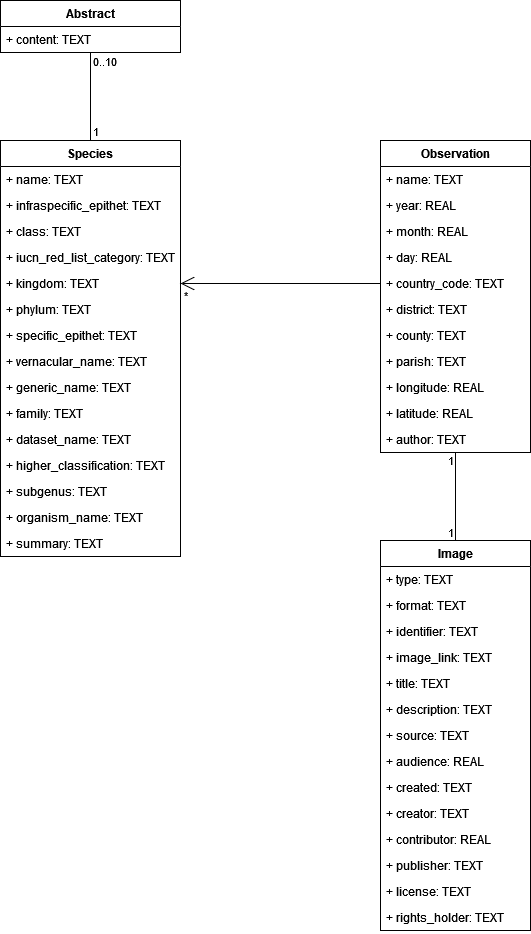
\includegraphics[width=0.5\linewidth]{figures/conceptual_data_model.drawio.png}
  \caption{Conceptual Data Model.}
  \Description{A Conceptual Data Model designed in UML, representing the main entities of the system.}
\end{figure}

\texttt{SPECIES} entity:
\begin{itemize}
    \item \texttt{name}: The name of the fungal species.
    \item \texttt{infraspecific\_epithet}: Additional taxonomic information specifying subspecies or variety.
    \item \texttt{class}: The taxonomic class of the species.
    \item \texttt{iucnRedList\_category}: The IUCN Red List category indicating the species' conservation status.
    \item \texttt{kingdom}: The taxonomic kingdom to which the species belongs.
    \item \texttt{phylum}: The taxonomic phylum of the species.
    \item \texttt{specific\_epithet}: Taxonomic information specifying the species within a genus.
    \item \texttt{vernacular\_name}: Common or colloquial name of the species.
    \item \texttt{generic\_name}: The generic or genus name to which the species belongs.
    \item \texttt{family}: The taxonomic family of the species.
    \item \texttt{dataset\_name}: Name of the dataset from which the species data originates.
    \item \texttt{higher\_classification}: Further taxonomic classification above the species level.
    \item \texttt{subgenus}: Taxonomic subgenus or subdivision.
    \item \texttt{organism\_name}: The name of the organism or species.
    \item \texttt{summary}: The summary of the Wikipedia page associated with the species.
\end{itemize}

\texttt{OBSERVATIONS} entity:
\begin{itemize}
    \item \texttt{name}: The name of the observed fungal species.
    \item \texttt{year}: The year of the observation.
    \item \texttt{month}: The month of the observation.
    \item \texttt{day}: The day of the observation.
    \item \texttt{country\_code}: The country code indicating the country of observation.
    \item \texttt{district}: The district where the observation took place.
    \item \texttt{county}: The county or regional division.
    \item \texttt{parish}: The specific parish or locality.
    \item \texttt{longitude}: The geographical longitude coordinates of the observation.
    \item \texttt{latitude}: The geographical latitude coordinates of the observation.
    \item \texttt{author}: The author or observer responsible for the observation.
\end{itemize}

\texttt{IMAGES} entity:
\begin{itemize}
    \item \texttt{type}: The type or category of the image.
    \item \texttt{format}: The file format or image format.
    \item \texttt{identifier}: An identifier for the image.
    \item \texttt{image\_link}: The link or reference to the image file.
    \item \texttt{title}: The title or caption associated with the image.
    \item \texttt{description}: A description or additional information about the image.
    \item \texttt{source}: The source or origin of the image.
    \item \texttt{audience}: The intended audience for the image.
    \item \texttt{created}: The date of creation or capture of the image.
    \item \texttt{creator}: The creator or author of the image.
    \item \texttt{contributor}: Contributions or additional contributors to the image.
    \item \texttt{publisher}: The publisher or source responsible for publishing the image.
    \item \texttt{license}: The license or usage terms associated with the image.
    \item \texttt{rights\_holder}: The rights holder or entity with rights to the image.
\end{itemize}

\texttt{ABSTRACT} entity:
\begin{itemize}
    \item \texttt{content}: The content of the abstract.
\end{itemize}

\subsubsection{\textbf{Data Pipeline}}

The data pipeline serves as the structured framework for our data preparation operations. It encompasses a sequence of designed steps to transform and refine raw data pertaining to fungal species, observations and content. Each stage within the pipeline fulfills a specific role, such as data extraction and cleansing. Conceptually, it operates as a structured workflow that systematically enhances the data's usability and accessibility. The figure below visually demonstrates the pipeline:

\begin{figure}[h]
  \centering
  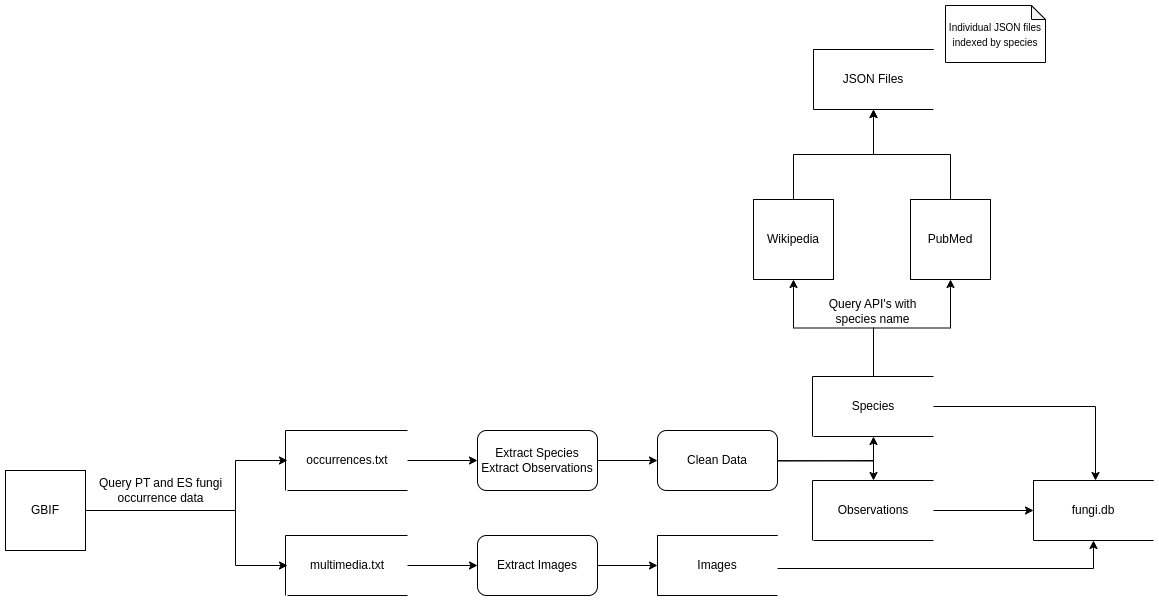
\includegraphics[width=\linewidth]{figures/data-flow-diagram.png}
  \caption{Data Pipeline.}
  \Description{The Data Pipeline, which demonstrates the order of operations on data.}
\end{figure}

To ensure that the entire data preparation process can be reliably recreated, the pipeline must be reproducible. In order to automate this process, a Makefile was designed. The Makefile enables us to automate and streamline the data preparation procedures from start to finish. 

% Section 3: Data Characterization
\subsection{Data Characterization}

% After analyzing the data collected for our project

% The following subsubsections summarize the data collected for our project and provide various statistics in order to better understand the 

An analysis was conducted in order to understand the characteristics of the collected data. In the following subsections, we present the results of this analysis as a summary of the data.

\subsubsection{\textbf{Document Presentation}}

In the final version of our project we aim to have two types of documents: one relative to a species and one relative to an observation.

The goal is to present the following information in the document relative to a species:
\begin{itemize}
    \item The species' taxonomic name, including: phylum, class, order, family, genus and species.
    \item Its vernacular name, if one exists.
    \item Its edibility.
    \item Its toxicity to humans.
    \item The number of observations of the given species present in our database, as well as an address to permit access to the documents of those observations.
    \item A catalog of images of observations of the species.
    \item An interactive map that summarily displays the location of said observations as well as the rough number per region.
    \item A list of abstracts of related scientific publications.
    \item The Wikipedia summary related to the species.
\end{itemize}

As for the document relative to an observation:
\begin{itemize}
    \item The latitude and longitude of the observation.
    \item The country, district, county and parish of the observation.
    \item The photographs associated with the observation, if present.
    \item The date of the observation.
    \item The name of the observer/rights-holder.
    \item The GBIF ID relative to the observation.
\end{itemize}

\subsubsection{\textbf{Descriptive and Exploratory Statistics}}

By plotting various graphics over the resulting data we were able to gain valuable insights on our document collection by visually representing complex information.

\begin{figure}[H]
    \centering
    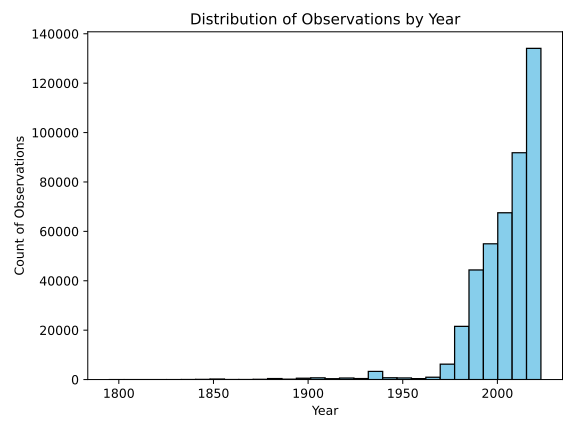
\includegraphics[width=0.6\linewidth]{figures/observation_distribution_by_year.png}
    \caption{Observations Distribution By Year}
\end{figure}

It is noticeable that the majority of the observations were registered over the 21st century and that the number of observations has been increasing over the past few decades. This could mean an increase in data accessibility and an improvement on fungus research and registration. Overall it seems to indicate good quality data as well as a tendency for more data to be available in the future.

\begin{figure}[H]
    \centering
    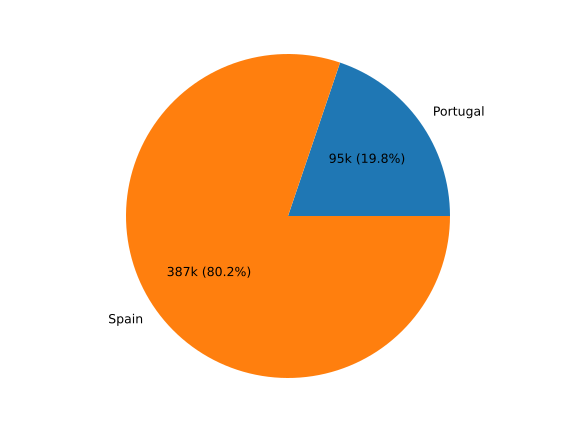
\includegraphics[width=0.6\linewidth]{figures/observation_distribution_by_country.png}
    \caption{Observations Count By Country}
\end{figure}

The number of registers available for Portugal and Spain seems to fairly represent the difference in area between these countries, so we conclude that the data adequately represents the diversity and characteristics of both countries, minimizing any potential bias.

\begin{figure}[H]
    \centering
    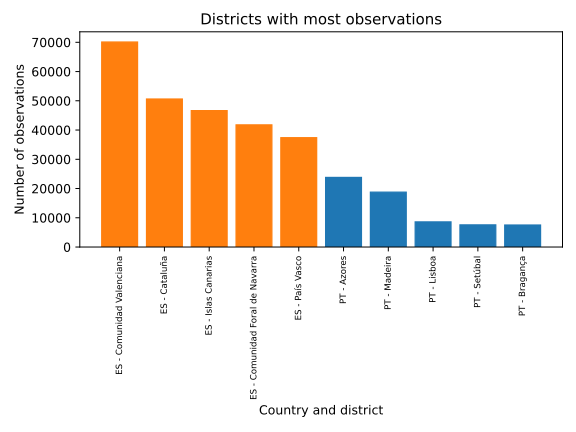
\includegraphics[width=0.6\linewidth]{figures/district_observations.png}
    \caption{Observations Distribution By District}
\end{figure}

As expected, the districts with most observations in Spain have a larger number of observations than the ones from Portugal. We can also observe that the archipelagos have the most observations from Portugal. 

\begin{figure}[H]
    \centering
    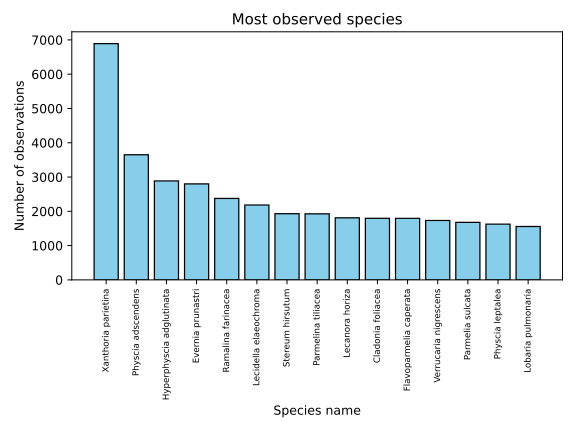
\includegraphics[width=0.6\linewidth]{figures/species_observations.png}
    \caption{Most Common Species}
\end{figure}

The 10 most frequent species' number of observations are all within the same order of magnitude.


% Section 4: Search Scenarios
\subsection{Search Scenarios} \label{search-scenarios}
Prospective search tasks and information needs are fundamental concepts in this type of project.

Information needs refer to the underlying reasons or motivations for conducting a search. They are the goals that users are trying to achieve when using an information retrieval system. These can vary widely, and might include tasks like finding specific facts, making decision, solving problems, or simply satisfying curiosity.

As an example, consider the following information needs:
\begin{itemize}
    \item[\textbf{IN1}] \textit{A user wants to research the toxic effects of fungi of the \textit{Amanita} genus.}
    \item[\textbf{IN2}] \textit{A user is looking for scientific articles or abstracts related to diseases associated with fungi species.}
\end{itemize}

To satisfy \textbf{IN1}, the user might start by entering a query like '\textit{toxic fungi}' onto our system. After submitting their query, the user will receive a list of search results, where they may find relevant information. There may be a scientific article which satisfies this exact need, which talks about toxic and poisonous fungi (for example, \textit{Pholiotina rugosa}). The abstract of said article may be within the reach of our system.



\section{Milestone 2 - Information Retrieval}

The second milestone focuses on the collection and indexing of data in the search engine, as well as the information retrieval process and it's subsequent evaluation. For this project, Apache Solr \cite{Solr} was chosen as a search platform. 

\subsection{Documents and Data Importing}

At the start of the current milestone, our data both stored in an SQLite database and JSON files. Considering that our database had a total of three tables, it was deemed appropriate to create an individual core for each entity. Additionally, it is important to note that the JSON files were storing information of up to 10 abstracts, as well as the summaries of the Wikipedia page of a species. Since these parameters differ on the type of information they provide to the user, it was also deemed appropriate to separate each one of them to their own collection, which led to the creation of two more cores. In total, we opted to define five types of documents, each one relative to a dedicated Apache Solr core:

\begin{itemize}
    \item \textbf{Species:} species-specific information
    \item \textbf{Observations:} observations-specific information
    \item \textbf{Images:} images-specific information
    \item \textbf{Abstracts:} abstracts related to a given species
    \item \textbf{Summaries:} summaries of wikipedia pages related to a given species
\end{itemize}


In order to start working with this information in Solr, the necessary cores were created and populated with the appropriate data. Given the proportions of our system, the uploaded data consisted of a small subset of the data at our disposal. This facilitated the future evaluation of our retrieval processes. However, it is important to note that the selected sample aimed to contain entities which were the most rich in information, avoiding duplicated and missing values.

For the creation of cores, and uploading of data, we resorted to the use of Solr's REST API.


\subsection{Indexing Schema}

Although Solr is able to automatically perform a set of operations to identify field types in the data imported, we found it helpful to create a customized schema for our documents to have more control over the search behaviour in our search system. To upload the custom schema we resorted again to Solr's REST API. This step should be done before populating the collection, so it can be properly indexed.

%TODO: fazer referencia a table no anexo

\begin{table*}
  \caption{Schema Types}
  \label{tab:schematypes}
  \begin{tabular}{lllp{2in}}
    \toprule
    Name&Class&Tokenizer&Filters\\
    \midrule
    \texttt{shortText}& \texttt{TextField}& \texttt{StandardTokenizerFactory}& \texttt{ASCIIFoldingFilterFactory, LowerCaseFilterFactory}\\
    \texttt{longText}& \texttt{TextField}& \texttt{StandardTokenizerFactory}& \texttt{ASCIIFoldingFilterFactory, LowerCaseFilterFactory, SynonymGraphFilterFactory, FlattenGraphFilterFactory}\\
    \texttt{mint}& \texttt{IntPointField}& \textit{N/A}& \textit{N/A}\\
    \texttt{mstring}& \texttt{StrField}& \textit{N/A}& \textit{N/A}\\
    \texttt{mdate}& \texttt{DateRangeField}& \textit{N/A}& \textit{N/A}\\
    \texttt{mdouble}& \texttt{DoublePointField}& \textit{N/A}& \textit{N/A}\\
    \bottomrule
  \end{tabular}
\end{table*}

We built a dedicated schema for each collection in our system. The created field types are detailed in table \ref{tab:schematypes}. Please see Appendix-\ref{sec:schema-definitions} for the definition of each schema. However, let's discuss the intricacies behind the \texttt{longText} type. It is used for text attributes with a significant length, namely for the contents of summaries or abstracts. At index time, the analyzer splits the words into tokens, performs ASCII folding, by removing accents and diacritics, and lower cases all characters. It proceeds to apply synonym expansion to the tokens, allowing multiple tokens with similar meaning to be associated with the same position in the token stream, and also flattens the token graph structure, transforming the graph structure into a linear structure. Similar operations are performed at query time, so that the resulting tokens match the indexed ones.

The default Solr schema typically allows multi-value fields, resulting in single-value lists for data like simple numerical values. This doesn't seem to impact search results, however we have specified single-value types for fields where it's applicable. We have chosen not to index all fields, as some were simply not relevant for search purposes, although they're still stored and retrieved in the search results.

Below you may find a detailed description of our schema's fields:



\subsection{Information Retrieval}

The query system provided by \texttt{Solr} has the purpose of fulfilling the information needs presented in section \ref{search-scenarios}. These can be translated into \texttt{eDisMax} queries. In order to demonstrate the efficacy of each boost type, we curated two distinct queries. Our selection is designed to underscore the practical utility and effectiveness in each boosting mechanism. The details of each query are documented in the following subsections. 

\subsubsection{\textbf{Query 1:} A user wants to research the toxic effects of fungi of the Amanita genus.} Initially, the user would simply filter the documents whose species have the genus \textit{Amanita}. Then, they could come up with some keywords related to their topic of search, like \textit{toxic}, \textit{toxicity}, or even \textit{poisonous}. Therefore, the computed query that satisfies this need could be:
\begin{verbatim}
species: amanita* 
AND 
content:'toxic'^2 content:'toxicity' content:'poisonous' content:'poison'
\end{verbatim}

The asterisk in \texttt{amanita*} is a wildcard character that represents zero or more characters, which means that species like \textit{Amanita muscaria} and \textit{Amanita phalloides} are included in the search. The content field looks for documents related to the keywords input by the user, namely those who match the terms \textit{toxic}, \textit{toxicity}, and \textit{poisonous}, giving more weight to \textit{toxic} due to the term boost attributed to it, specified by the \texttt{\^{}2} after it.

\subsubsection{\textbf{Query 2:} A user is looking for scientific articles or abstracts related to diseases associated with fungi species.} The computed query that satisfies this need could simply be \texttt{content:'disease'}, which looks for documents that match the term \textit{disease}. However, since the \texttt{content} field is equipped with a synonym filter, the retrieved documents will not only match this term, but also the defined synonyms, like \textit{illness}, \textit{sickness}, \textit{disorder}, \textit{condition}, and \textit{malady}, which increases the overall number of relevant retrieved documents.


\subsection{Evaluation}

In order to evaluate the performance of our queries we compare a manually selected list of relevant documents with the ones returned by the system. To assess the improvements provided by our schema, we compared it to a simpler counterpart, using only lower case filters. The metrics utilized to compare our schema to the simpler one are a \textbf{Precision-Recall Curve}, the average precision and precision at 10, which are described below.


\begin{itemize}
    \item Average Precision (AP): The average of the precision values obtained for the set of top N documents existing each time a new relevant document is retrieved.
    \item Precision at 10 (P@10): Precision at a specific cut point in the result ranked list, in this case 10, i.e. the ratio of the first 10 values that are relevant.
    \item Precision-Recall Curve: A graph that illustrates how precision varies according to recall, providing insights into how the system performs at varying degrees of scrutiny.

\end{itemize}

\textbf{Query 1}

Below are present the evaluation result's for the simpler schema:

\begin{center}
\begin{tabular}{lll}
\toprule
 &                  Metric &    Value \\
\midrule
1 &       Average Precision &  0.817857 \\
2 &  Precision at 10 (P@10) &      0.6 \\
\bottomrule
\end{tabular}
\end{center}

\begin{figure}[H]
    \centering
    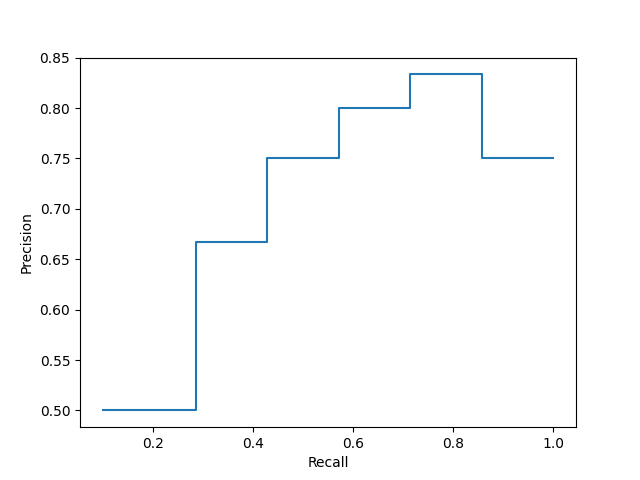
\includegraphics[width=0.6\linewidth]{figures/toxic_simple.png}
    \caption{Simple schema's Precision-Recall Curve}
\end{figure}

As we can see below, the boosting had a noticeable effect on the performance of our system:

\begin{center}
\begin{tabular}{lll}
\toprule
 &                  Metric &    Value \\
\midrule
1 &       Average Precision &  0.97619 \\
2 &  Precision at 10 (P@10) &      0.6 \\
\bottomrule
\end{tabular}
\end{center}

\begin{figure}[H]
    \centering
    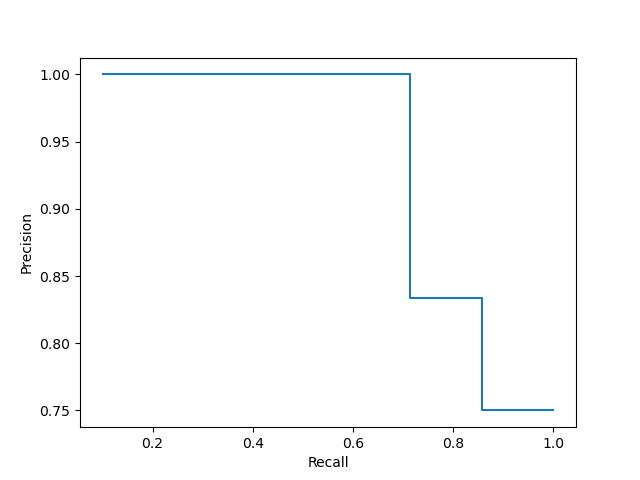
\includegraphics[width=0.6\linewidth]{figures/toxic.png}
    \caption{Refined schema's Precision-Recall Curve}
\end{figure}



\textbf{Query 2}

Again, below are presented the performance results for the simpler schema:

\begin{center}
\begin{tabular}{lll}
\toprule
 &                  Metric &    Value \\
\midrule
1 &       Average Precision &  0.877381 \\
2 &  Precision at 10 (P@10) &       0.6 \\
\bottomrule
\end{tabular}
\end{center}

\begin{figure}[H]
    \centering
    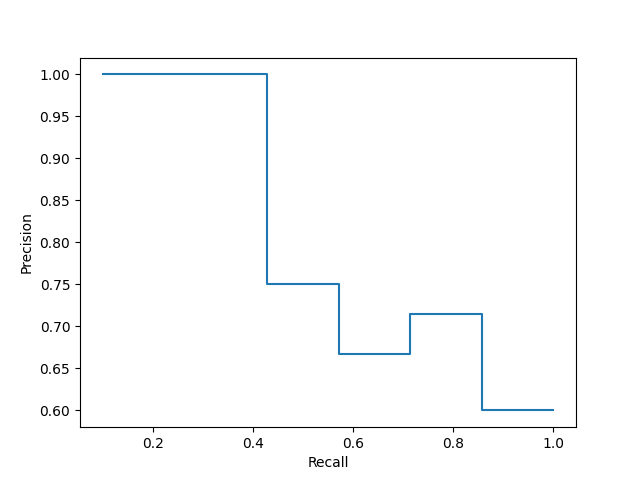
\includegraphics[width=0.6\linewidth]{figures/disease_simple.png}
    \caption{Simple schema's Precision-Recall Curve}
\end{figure}

Finally, the performance results for the refined schema:

\begin{center}
\begin{tabular}{lll}
\toprule
 &                  Metric &    Value \\
\midrule
1 &       Average Precision &  0.930556 \\
2 &  Precision at 10 (P@10) &       0.6 \\
\bottomrule
\end{tabular}
\end{center}

\begin{figure}[H]
    \centering
    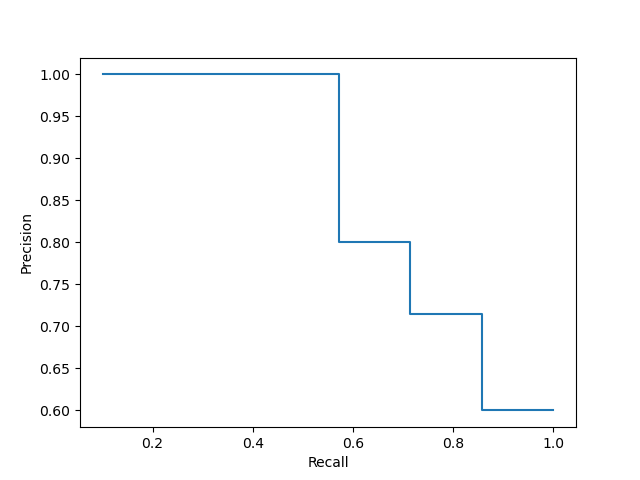
\includegraphics[width=0.6\linewidth]{figures/disease.png}
    \caption{Refined schema's Precision-Recall Curve}
\end{figure}







% Section 5: Conclusion
\section{Conclusion}

After selecting the source and datasets to be used, cleaning and processing the data, our pipeline returns a collection of documents containing valuable information to be used in our search system. The search platform using this collection, with customized indexation and tools for information retrieval is able to return relevant information, as we've evaluated in accordance to the user's information needs. There is room for future improvement, such as refining the information retrieval process, making the search system more robust, or even broadening the search possibilities through additional data or features.

\newpage
\appendix
\section{Schema definitions}\label{sec:schema-definitions}

\begin{table}[H]
  \caption{Schema for the 'abstracts' collection}
  \label{tab:abstracts-schema}
  \begin{tabular}{lll}
    \toprule
    name&type&indexed\\
    \midrule
    \texttt{abstract\_id} & \texttt{mint} & \texttt{false} \\
    \texttt{species}&\texttt{shortText}&\texttt{true}\\
    \texttt{content}&\texttt{longText}&\texttt{true}\\
  \bottomrule
\end{tabular}
\end{table}

\begin{table}[H]
  \caption{Schema for the 'images' collection}
  \label{tab:images-schema}
  \begin{tabular}{lll}
    \toprule
    name & type & indexed \\
    \midrule
    \texttt{index} & \texttt{mint} & \texttt{false} \\
    \texttt{gbif\_id} & \texttt{mint} & \texttt{true} \\
    \texttt{type} & \texttt{mstring} & \texttt{false} \\
    \texttt{format} & \texttt{mstring} & \texttt{true} \\
    \texttt{identifier} & \texttt{mstring} & \texttt{false} \\
    \texttt{image\_link} & \texttt{mstring} & \texttt{false} \\
    \texttt{title} & \texttt{shortText} & \texttt{true} \\
    \texttt{description} & \texttt{shortText} & \texttt{true} \\
    \texttt{source} & \texttt{shortText} & \texttt{true} \\
    \texttt{audience} & \texttt{shortText} & \texttt{true} \\
    \texttt{contributor} & \texttt{shortText} & \texttt{true} \\
    \texttt{publisher} & \texttt{shortText} & \texttt{true} \\
    \texttt{license} & \texttt{shortText} & \texttt{false} \\
    \texttt{created} & \texttt{mdate} & \texttt{true} \\
    \texttt{creator} & \texttt{shortText} & \texttt{true} \\
    \texttt{rightsHolder} & \texttt{shortText} & \texttt{true} \\
    \bottomrule
  \end{tabular}
\end{table}

\begin{table}[H]
  \caption{Schema for the 'observations' collection}
  \label{tab:observations-schema}
  \begin{tabular}{llll}
    \toprule
    name & type & indexed & stored \\
    \midrule
    \texttt{index} & \texttt{mint} & \texttt{false} & \\
    \texttt{species} & \texttt{shortText} & \texttt{true} & \\
    \texttt{gbif\_id} & \texttt{mint} & \texttt{true} & \\
    \texttt{date} & \texttt{pdate} & \texttt{true} & \texttt{true} \\
    \texttt{country\_code} & \texttt{mstring} & \texttt{true} & \\
    \texttt{district} & \texttt{shortText} & \texttt{true} & \\
    \texttt{county} & \texttt{shortText} & \texttt{true} & \\
    \texttt{parish} & \texttt{shortText} & \texttt{true} & \\
    \texttt{longitude} & \texttt{mdouble} & \texttt{true} & \\
    \texttt{latitude} & \texttt{mdouble} & \texttt{true} & \\
    \texttt{author} & \texttt{shortText} & \texttt{true} & \\
    \bottomrule
  \end{tabular}
\end{table}


\begin{table}[H]
  \caption{Schema for the 'summaries' collection}
  \label{tab:summaries-schema}
  \begin{tabular}{lll}
    \toprule
    name & type & indexed \\
    \midrule
    \texttt{summary\_id} & \texttt{mint} & \texttt{false} \\
    \texttt{species} & \texttt{shortText} & \texttt{true} \\
    \texttt{content} & \texttt{longText} & \texttt{true} \\
    \bottomrule
  \end{tabular}
\end{table}

\begin{table}[H]
  \caption{Schema for the 'species' collection}
  \label{tab:species-schema}
  \begin{tabular}{lll}
    \toprule
    name & type & indexed \\
    \midrule
    \texttt{index} & \texttt{mint} & \texttt{false} \\
    \texttt{species} & \texttt{shortText} & \texttt{true} \\
    \texttt{infraspecificEpithet} & \texttt{mstring} & \texttt{true} \\
    \texttt{class} & \texttt{mstring} & \texttt{true} \\
    \texttt{iucnRedListCategory} & \texttt{mstring} & \texttt{true} \\
    \texttt{kingdom} & \texttt{mstring} & \texttt{true} \\
    \texttt{phylum} & \texttt{mstring} & \texttt{true} \\
    \texttt{specificEpithet} & \texttt{mstring} & \texttt{true} \\
    \texttt{vernacularName} & \texttt{mstring} & \texttt{true} \\
    \texttt{genericName} & \texttt{mstring} & \texttt{true} \\
    \texttt{family} & \texttt{mstring} & \texttt{true} \\
    \texttt{higherClassification} & \texttt{mstring} & \texttt{true} \\
    \texttt{subgenus} & \texttt{mstring} & \texttt{true} \\
    \texttt{organismName} & \texttt{mstring} & \texttt{true} \\
    \texttt{datasetName} & \texttt{shortText} & \texttt{false} \\
    \bottomrule
  \end{tabular}
\end{table}


%%
%% The next two lines define the bibliography style to be used, and
%% the bibliography file.
\bibliographystyle{ACM-Reference-Format}
\bibliography{samples/pri}


%%
%% If your work has an appendix, this is the place to put it.



\end{document}
\endinput
%%
%% End of file `sample-sigconf.tex'.
